\documentclass[a4paper]{article}
\usepackage{tikz}
\usetikzlibrary{petri,arrows}
\usepackage{amstext}

\begin{document}


%% TikZ style options %%
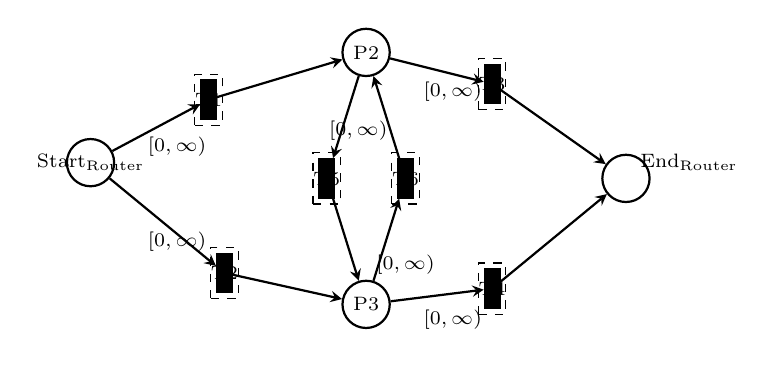
\begin{tikzpicture}[font=\scriptsize, xscale=1, yscale=1]
%% the figure can be scaled by changing xscale and yscale
%% positions of place/transition labels that are currently fixed to label=135 degrees
%% can be adjusted so that they do not cover arcs
%% similarly the curving of arcs can be done by adjusting bend left/right=XX
%% labels may be slightly skewed compared to the tapaal drawing due to rounding.
%% This can be adjusted by tuning the coordinates of the label
\tikzstyle{arc}=[->,>=stealth,thick]
\tikzstyle{transportArc}=[->,>=diamond,thick]
\tikzstyle{inhibArc}=[->,>=o,thick]
\tikzstyle{every place}=[minimum size=6mm,thick]
\tikzstyle{every transition} = [fill=black,minimum width=2mm,minimum height=5mm]
\tikzstyle{every token}=[fill=white,text=black]
\tikzstyle{sharedplace}=[place,minimum size=7.5mm,dashed,thin]
\tikzstyle{sharedtransition}=[transition, fill opacity=0, minimum width=3.5mm, minimum height=6.5mm,dashed]
\tikzstyle{urgenttransition}=[place,fill=white,minimum size=2.0mm,thin]\tikzstyle{uncontrollabletransition}=[transition,fill=white,draw=black,very thick]
%% TikZ-figure elements %%
\node[place] at (4.1,-1.9) (Start_Router) {};
%% label for place Start_Router
\draw (4.1,-1.9) node[align=left] {$\mathrm{Start_{Router}}$};
\node[place] at (7.6,-0.5) (P2) {};
%% label for place P2
\draw (7.6,-0.5) node[align=left] {$\mathrm{P2}$};
\node[place] at (7.6,-3.7) (P3) {};
%% label for place P3
\draw (7.6,-3.7) node[align=left] {$\mathrm{P3}$};
\node[place] at (10.9,-2.1) (End_Router) {};
%% label for place End_Router
\draw (11.7,-1.9) node[align=left] {$\mathrm{End_{Router}}$};
\node[transition] at (5.6,-1.1) (T1) {};
\node[sharedtransition] at (T1.center) { };
%% label for transition T1
\draw (5.6,-1.1) node  {$\mathrm{T1}$};
\node[transition] at (5.8,-3.3) (T2) {};
\node[sharedtransition] at (T2.center) { };
%% label for transition T2
\draw (5.8,-3.3) node  {$\mathrm{T2}$};
\node[transition] at (9.2,-0.9) (T3) {};
\node[sharedtransition] at (T3.center) { };
%% label for transition T3
\draw (9.2,-0.9) node  {$\mathrm{T3}$};
\node[transition] at (9.2,-3.5) (T4) {};
\node[sharedtransition] at (T4.center) { };
%% label for transition T4
\draw (9.2,-3.5) node  {$\mathrm{T4}$};
\node[transition] at (7.1,-2.1) (T5) {};
\node[sharedtransition] at (T5.center) { };
%% label for transition T5
\draw (7.1,-2.1) node  {$\mathrm{T5}$};
\node[transition] at (8.1,-2.1) (T6) {};
\node[sharedtransition] at (T6.center) { };
%% label for transition T6
\draw (8.1,-2.1) node  {$\mathrm{T6}$};
\draw[arc] (Start_Router) to[bend right=0] (T1) {};
%% Label for arc between Start_Router and T1
\draw (5.2,-1.7) node {$\mathrm{[0,\infty)}$};
\draw[arc] (T1) to[bend right=0] (P2) {};
\draw[arc] (Start_Router) to[bend right=0] (T2) {};
%% Label for arc between Start_Router and T2
\draw (5.2,-2.9) node {$\mathrm{[0,\infty)}$};
\draw[arc] (T2) to[bend right=0] (P3) {};
\draw[arc] (P2) to[bend right=0] (T3) {};
%% Label for arc between P2 and T3
\draw (8.7,-1.0) node {$\mathrm{[0,\infty)}$};
\draw[arc] (T3) to[bend right=0] (End_Router) {};
\draw[arc] (P3) to[bend right=0] (T4) {};
%% Label for arc between P3 and T4
\draw (8.7,-3.9) node {$\mathrm{[0,\infty)}$};
\draw[arc] (T4) to[bend right=0] (End_Router) {};
\draw[arc] (P2) to[bend right=0] (T5) {};
%% Label for arc between P2 and T5
\draw (7.5,-1.5) node {$\mathrm{[0,\infty)}$};
\draw[arc] (T5) to[bend right=0] (P3) {};
\draw[arc] (P3) to[bend right=0] (T6) {};
%% Label for arc between P3 and T6
\draw (8.1,-3.2) node {$\mathrm{[0,\infty)}$};
\draw[arc] (T6) to[bend right=0] (P2) {};
\end{tikzpicture}
\end{document}
